%%%%%%%%%%%%%%%%%%%%%%%%%%%%%%%%%%%%%%%%%
% Thesis 
% LaTeX Template
% Version 1.2 (29/7/12)
%
% This template has been downloaded from:
% http://www.latextemplates.com
%
% Original authors:
% Steven Gunn 
% http://users.ecs.soton.ac.uk/srg/softwaretools/document/templates/
% and
% Sunil Patel
% http://www.sunilpatel.co.uk/thesis-template/
%
% License:
% CC BY-NC-SA 3.0 (http://creativecommons.org/licenses/by-nc-sa/3.0/)
%
% Note:
% Make sure to edit document variables in the Thesis.cls file
%
%%%%%%%%%%%%%%%%%%%%%%%%%%%%%%%%%%%%%%%%%

%----------------------------------------------------------------------------------------
%	PACKAGES AND OTHER DOCUMENT CONFIGURATIONS
%----------------------------------------------------------------------------------------

\documentclass[11pt, a4paper, oneside]{Thesis} % Paper size, default font size and one-sided paper

\graphicspath{{./Pictures/}} % Specifies the directory where pictures are stored

\usepackage[square, numbers, comma, sort&compress]{natbib} % Use the natbib reference package - read up on this to edit the reference style; if you want text (e.g. Smith et al., 2012) for the in-text references (instead of numbers), remove 'numbers' 
\hypersetup{urlcolor=black, colorlinks=true} % Colors hyperlinks in blue - change to black if annoying
\title{\ttitle} % Defines the thesis title - don't touch this
\def\theartefact{madame}
\def\Theartefact{Madame}
\def\THEARTEFACT{MADAME}
\begin{document}

\frontmatter % Use roman page numbering style (i, ii, iii, iv...) for the pre-content pages

\setstretch{1.5} % Line spacing of 1.3

% Define the page headers using the FancyHdr package and set up for one-sided printing
\fancyhead{} % Clears all page headers and footers
\rhead{\thepage} % Sets the right side header to show the page number
\lhead{} % Clears the left side page header

\pagestyle{fancy} % Finally, use the "fancy" page style to implement the FancyHdr headers

\newcommand{\HRule}{\rule{\linewidth}{0.5mm}} % New command to make the lines in the title page

% PDF meta-data
\hypersetup{pdftitle={\ttitle}}
\hypersetup{pdfsubject=\subjectname}
\hypersetup{pdfauthor=\authornames}
\hypersetup{pdfkeywords=\keywordnames}

%----------------------------------------------------------------------------------------
%	TITLE PAGE
%----------------------------------------------------------------------------------------

\begin{titlepage}
\begin{center}

\includegraphics[width=8cm]{Figures/uib-emblem-svart} \\[0.5cm]
% 
\includegraphics{uib-emblem-svart}\vfill % University/department logo - uncomment to place it
\textsc{\LARGE \univname}\\[1.5cm] % University name
\textsc{\Large Master Thesis}\\[0.5cm] % Thesis type

\HRule \\[0.4cm] % Horizontal line
{\huge \bfseries \ttitle}\\[0.4cm] % Thesis title
\HRule \\[1.5cm] % Horizontal line
 
\begin{minipage}{0.4\textwidth}
\begin{flushleft} \large
\emph{Author:}\\
\href{http://elseth.me}{\authornames} % Author name - remove the \href bracket to remove the link
\end{flushleft}
\end{minipage}
\begin{minipage}{0.4\textwidth}
\begin{flushright} \large
\emph{Supervisor:} \\
{\supname} % Supervisor name - remove the \href bracket to remove the link  
\end{flushright}
\end{minipage}\\[2cm]
 
% \large \textit{A thesis submitted in fulfilment of the requirements\\ for the degree of \degreename}\\[0.3cm] % University requirement text
\textit{in the}\\[0.1cm]
\groupname\\\deptname\\[0.5cm] % Research group name and department name
 
{\large \today}\\[1cm] % Date
\end{center}

\end{titlepage}

%----------------------------------------------------------------------------------------
%	QUOTATION PAGE
%----------------------------------------------------------------------------------------

\pagestyle{empty} % No headers or footers for the following pages

\null\vfill % Add some space to move the quote down the page a bit

\textit{``It depends upon what the meaning of the word 'is' is"}

\begin{flushright}
-- Bill Clinton
\end{flushright}

\vfill\vfill\vfill\vfill\vfill\vfill\null % Add some space at the bottom to position the quote just right

\clearpage % Start a new page

%----------------------------------------------------------------------------------------
%	ABSTRACT PAGE
%----------------------------------------------------------------------------------------

\addtotoc{Abstract} % Add the "Abstract" page entry to the Contents

\abstract{\addtocontents{toc}{\vspace{1em}} % Add a gap in the Contents, for aesthetics
In this thesis I will describe the methods used in creating the artefact: \theartefact\ \Theartefact\ \THEARTEFACT\ 
}

\clearpage % Start a new page

%----------------------------------------------------------------------------------------
%	ACKNOWLEDGEMENTS
%----------------------------------------------------------------------------------------

\setstretch{1.5} % Reset the line-spacing to 1.3 for body text (if it has changed)

\acknowledgements{\addtocontents{toc}{\vspace{1em}} % Add a gap in the Contents, for aesthetics
TODO
}
\clearpage % Start a new page

%----------------------------------------------------------------------------------------
%	LIST OF CONTENTS/FIGURES/TABLES PAGES
%----------------------------------------------------------------------------------------

\pagestyle{fancy} % The page style headers have been "empty" all this time, now use the "fancy" headers as defined before to bring them back

\lhead{\emph{Contents}} % Set the left side page header to "Contents"
\tableofcontents % Write out the Table of Contents

\lhead{\emph{List of Figures}} % Set the left side page header to "List of Figures"
\listoffigures % Write out the List of Figures

\lhead{\emph{List of Tables}} % Set the left side page header to "List of Tables"
\listoftables % Write out the List of Tables

%----------------------------------------------------------------------------------------
%	ABBREVIATIONS
%----------------------------------------------------------------------------------------

\clearpage % Start a new page

\setstretch{1.5} % Set the line spacing to 1.5, this makes the following tables easier to read

\lhead{\emph{Abbreviations}} % Set the left side page header to "Abbreviations"
\listofsymbols{ll} % Include a list of Abbreviations (a table of two columns)
{
\textbf{ACC} & \textbf{A}ctivity \textbf{C}entric \textbf{C}omputing \\
\textbf{UI} & \textbf{U}ser \textbf{I}nterface \\
\textbf{HCI} & \textbf{H}uman-\textbf{C}omputer \textbf{I}nteraction \\
%\textbf{Acronym} & \textbf{W}hat (it) \textbf{S}tands \textbf{F}or \\
}

%----------------------------------------------------------------------------------------
%	DEDICATION
%----------------------------------------------------------------------------------------

% \setstretch{1.5} % Return the line spacing back to 1.3

% \pagestyle{empty} % Page style needs to be empty for this page

% \dedicatory{For/Dedicated to/To my\ldots} % Dedication text

% \addtocontents{toc}{\vspace{2em}} % Add a gap in the Contents, for aesthetics

%----------------------------------------------------------------------------------------
%	THESIS CONTENT - CHAPTERS
%----------------------------------------------------------------------------------------

\mainmatter % Begin numeric (1,2,3...) page numbering

\pagestyle{fancy} % Return the page headers back to the "fancy" style

% Include the chapters of the thesis as separate files from the Chapters folder
% Uncomment the lines as you write the chapters

% Chapter Template

\chapter{Introduction} % Main chapter title

\label{Introduction}
%use \ref{Introduction}

\lhead{Chapter \ref{Introduction}. \emph{Introduction}} % Change X to a consecutive number; this is for the header on each page - perhaps a shortened title

%----------------------------------------------------------------------------------------
%	SECTION 1: Background
%----------------------------------------------------------------------------------------

% \section{Background} Should this be used as the main introduction before the motivation? ala Aleksander Larsen
The Internet is now an ingrained part of our everyday life,
and the amount of content and services that are available through it is growing at an ever increasing rate.
For all this information to be of use to humans it is necessary to have some interface through which to access the parts of it that are relevant to us.
\citet{Shirky2007} tells of the early attempts to structure the Web,
using ontologies and hierarchies created by experts.
This soon got clunky as the number of documents increased,
and this way of organizing information fell out of favor to be replaced by searching for information using keywords.
It is this phase of organizing information we are in now.

\citet{Berners-Lee2001} suggested that we could do better than keyword matching.
With searching as it works today users have to manually check the results from the search engine,
and compare the results from several documents, following links as is necessary.
Instead of forcing users to go through this process,
this new idea was to enrich the documents we put on the Web with metadata that could be read and reasoned about by computers.
By doing this we could move the tedious task of siphoning though Web sites looking for relevant information from users
over to specialized software agents that could collect information on the topic and return the answer to the user.

This does create some extra work for content creators on the Internet.
Adding metadata to content is not a trivial task.
The W3C recommends using RDFa to add metadata \citep{Pemberton:08:RXS}.
But to use RDFa the user not only needs to know the syntax of RDFa itself,
but also which ontologies exists that contain the meaning the creator wants to convey,
and knowledge about how those ontologies are structured to use them in the correct way.

Ontology is the philosophical discipline of finding out which things exist,
the manner in which one can say that these exist and how these can be categorized.
When talking about ontologies in the context of the Semantic Web,
an ontology can be explained as a collection of things that one can describe using the ontology,
and how these things can relate to each other.

%----------------------------------------------------------------------------------------
%	SECTION 2: Motivation
%----------------------------------------------------------------------------------------

\section{Motivation}
According to \citet{Gantz2011} the amount of information in the world now doubles every two years.
Should this trend continue, we are going to need better ways of searching through all the information that is generated.
We are going to need to be able to search for content in a way that lets us search for concepts, not only keywords.
What we want is to have linked semantic data that help move the burden of finding relevant content from us over to machines.

At the moment, adding semantic markup to Web sites is unfeasible for most content creators on the Web.
Adding proper metadata does not only mean that you need to know HTML,
but also that you need to understand the concept of ontologies, and know of the different ontologies that exist.
In addition you need to know of the implementation of \nom{RDFa}{Resource Description Framework in attributes}, microdata or microformats
as well as the content of the specific ontologies you intent to use on your site.

Adding metadata shouldn't really be that hard.
Humans are good at knowing what things are.
We know what the things on Web sites mean, and which concepts they are meant to convey.
Natural language is mainly ambiguous to computers, not human beings.
I want to create a tool that lets users use their knowledge of natural language and the concepts it conveys
to create metadata by disambiguating the language for the computer, and letting it create the mappings and the elements on the Web page.

The aim of this thesis will be to develop a prototype artefact that will let users add metadata to Web pages using natural language.
The prototype should map to the schema.org ontology,
as using this ontology can increase the visibility of the Web page in search results in the most popular search engines.
The tool should also be able to express meaning in other ontologies, so that it can help create a rich Web of interconnected data.

The prototype tool will be created using Node.js\footnote{\url{http://nodejs.org}},
a JavaScript platform based on Google Chromes JavaScript runtime,
and using MongoDB\footnote{\url{http://www.mongodb.org}} as a database solution.
JavaScript is a good language to rapidly create prototypes, and the flexibility and simplicity inherent in using the same language
server side, client side and in database communication, inspired me to try using and learning these tools for the thesis.

%It is estimated that the amount of information created by humans before 2005,
%
%is smaller that the amount of information created after 2005.

I choose to develop using node.js because it's a new and exciting technology that would make it possible to write
the entire app using one programming language for front-end, server side and as the database query language.

Creating a Web application allows the work to consist both of back end server side components, and front-end work.

%----------------------------------------------------------------------------------------
%	SECTION 3: Research Questions
%----------------------------------------------------------------------------------------

\section{Research question}
The main research question in this thesis is:

\emph{"Is it possible to create a tool which allows naïve users to easily add metadata to their Web sites using natural language?"}

In this context we should understand "naïve users" as users who do not have any training in the use of semantic technologies,
and who do not have any knowledge about the ontologies used for testing in this thesis.

To answer this question I will develop a tool called \theartefact, a play on the goal "MetADAta MAde Easy".
The tool will consist of a logical backend tied to a Web front-end,
and the different modules will be created in an iterative way to get working proofs of concepts for testing early.

There are several sub questions that will need to examined to answer this question.
\begin{itemize}
	\item How should users pick the parts of a Web page they want to add metadata to, and find the concepts it describes using natural language?
	\item Is WordNet suitable for representing disambiguated concepts from natural language in a way that will allow us to map these concepts to formal ontologies?
	\item How should an algorithm be implement to finds mappings from the natural language concept to types in
			formal ontologies in a way that preserves the semantic content of the concept?
	\item Is it possible to add metadata to Web pages in such a way that it does not change the way the page is rendered by browsers?
\end{itemize}

In addition I will also need to solve the technical problems of how to import and export Web pages from the artefact,
and how to save the resulting documents on the server.

\section{Target audience}
The main goal of the work with \theartefact\ is to lower the barrier of entry for enhancing Web sites with metadata.
I want to make metadata accessible to content creators on the Web that do not know enough about Semantic Web technologies
to add this data them selves.

Due to availability of English natural language resources this thesis will focus development on mapping English text,
and limit the target group to users who write content in English.
I will also assume that the users control the HTML of their Web pages,
and that being provided with a new HTML document will allow the user to update their documents.


% Chapter Template

\chapter{Theory} % Main chapter title

\label{Theory} % Change X to a consecutive number; for referencing this chapter elsewhere, use \ref{ChapterX}

\lhead{Chapter \ref{Theory}. \emph{Theory}} % Change X to a consecutive number; this is for the header on each page - perhaps a shortened title

\section{Ontology and folksonomy}
One of the central concepts in semantic web technology is that of the ontology. 
In philosophy Ontology is the branch dealing with the study of which things 'exists', and if it is possible to categorize these things. 
For artificial intelligence \citet{Gruber1993} explained it as "an explicit specification of a conceptualization". 
That is than one commits to a given conceptualization of the domain in question, and formalize how we describe and reason about these conceptualizations. 
\citet{Pretorius2004} also gives a good overview of the history of the term, and show several of the interpretations and formalisms. 
One can also go to \citet{Noy1997} to find comparisons of several of the early ontologies, including WordNet which will be important in this thesis.

\citet{Shirky2007} criticizes the use of ontologies as a way of trying to enforce a structure on something that is by nature unstructured. 
He instead pushes the idea of common tagging. 
Part of the reason he criticizes the ontology approach is that it seem improbable that experts can know the needs of all the users a priori, and therefor that every ontology will prove to be inadequate.
%\citet{Doan2002} Tror ikke denne skal brukes
On the semantic web, ontologies are represented using collection of RDF( Resource Description Framework) triplets. 
These triplets are in the form of <subject, predicate, object>, much like simple declarative sentences \citep{Berners-Lee2001}. 
Each subject and predicate, and some objects, is represented by an URI( Universal Resource Identifier), which links to the resource that describes it.

While ontologies are formally constructed taxonomies, folksonomies are informal taxonomies generated by collecting tags or annotations from collaborative tagging systems on a given platform\citep{Tang2009}. 
\citet{Mika2005} has given a more formal definition of folksonomy where he sees a folksonomy as a set of tags T, 
$T \subseteq A \times C \times I$, where A is the set of users tagging, C is the set of tags, and I is the set of objects being tagged.
\citet{Gruber2007} suggested that one should add the source of the tag, and some kind of rating system to help filter out junk tags. 
\citet{Scerri2008} on the other hand suggests removing the objects being tagged from the ontology, 
seeing that the objects that are being described are not part of the tool to describe them.
Instead they like Gruber want to add the source of the tag, the number or times a tag occur, and the tagging behavior of each user.
\citet{Bang2008} explains the difference between ontologies and folksonomies by classifying them as a priori and a posteriori annotations. 
That is, ontologies are created by experts as ways on conceptualizing a domain, folksonomies on the other hand are samples of how people speak or think about a domain.
Folksonomies grew as a subject of research as it became popular for users to tag content on the internet with keywords they felt were relevant.

For users tags are convenient, since Adding additional tags can make it easier for humans to search and browse collections. This is especially true for multimedia content, which we don't yet have good tools for searching in \citep{Weinberger2008}.
Tags provide meta data about content in a way that makes sense to humans. From an information retrieval perspective this is interesting since it means that humans in some way add meaning to the content.
There however are several problems with using tags as the basis of a semantic web. \citet{Tang2009} mention several. 
Tags are supposed to be written in natural language, and natural language has words that are synonymes(words that are written in different ways, 
but mean the same), homonymes(words with different meanings that are written in the same way), or polynyms( a word that can have several meanings) 
making it unsuitable for computer reasoning since they are ambiguous \citep{Passant2008}. 
As \citet{Golder2005} mentions, users also operate on different levels of abstraction, which can make it harder to find interesting resources.
In addition to this comes the problem of non dictionary words, both new, or compound words, or simply words that have been misspelled\citep{Tonkin2006}.


There has been done a lot of research into how one can lift semantic data out of these unstructured tags.
\citet{Golder2005} has done research into the statistical analysis of tags. 
The analysis done here show that there seems to develop vocabularies of frequently used tags. 
This might help diminish the effect of misspelled and nonsense words. Similar findings were also reported by \citep{Shirky2007}

There has also been done research into automatic clustering. 
\citet{Mika2005} created clusters by creating weighted graphs, and compared using tag concurrence and actor interest as weights.  
\citet{Brooks2006} has done work an categorizing blogs entries by tags, to see if concurrence of tags indicated similar content. 
Using the most common tags did give some results, but only broad categories. The results were not better than extracting words that were given asserted to be relevant for the category.

\citep{Tang2009} tries to go further that clustering tags, and tries to build an hierarchical model from a folksonomy. 
They use a probabilistic model that takes into account the frequency and concurrence of tags and tries to generalize it to an ontology. 
The method does get good results in creating the hierarchy, but does also show som inappropriate sub/super category inferences.

\citet{Weinberger2008} suggests a method for removing ambiguity from tags,
 by suggesting additional tags to the user when the tag entered can belong to one of several distinct sets 

While there are many difficulties attached to merging the social and semantic web, and with lifting semantic data from tags, there are many researchers who stress the need for this \citep{Passant2007,Mika2005, Gruber2007}.

\section{WordNet and lexitags}
\label{TheoryWordNet}
Lexitags \citep{Veres2011} utilizes a different approach for getting semantic meaning out of tags that the approaches mentioned until now. 
Instead of analyzing existing folksonomies and try to lift semantic data out of these tags, the idea presented is to turn it around and make users attach meaning to the tags at input time.
This is done by letting users disambiguate the tags by using WordNet synsets, an idea that was also mentioned by.

WordNet is a lexical reference system that stores words in sets of synonymes called synsets. The idea is to separate the word form from the word sense. 
The underlying assumption is that the user already knows English, is familiar with the concepts that are conveyed, 
and doesn't need definitions to understand, but can use synonymes to identify the meaning they want to convey\citep{Miller1990}.

In addition to storing these synsets WordNet also contains information about the semantic relationship between different concepts. 
The synonymy relationship is obviously contained within each synset, 
though it should be mentioned that the definition used in WordNet is not one where substitution never changes the truth value of a sentence. 
WordNet uses a weaker definition where two word forms can be seen as synonymes in relation to some semantic context. 
The antonymy relationship is another relationship between word forms. While the exact definition of antonymy is hard to pin down, the intuitive notion that an antonym to x is not-x will take us a long way\citep{Miller1990}.

WordNet also stores information about hyponymy and hypernymy, which is a relationship between concepts.
 A hypernym can be explained as a generalization of some concept, a hyponym on the other hand can be seen as a specialization of a concept. 
 \{tree\} can for example be seen as a hyponym of \{plant\}, and the reverse relation is a hypernymy relation \citep{Veres2010}.

The fact that WordNet separates sense and form is good for our purposes, as we are interested in the sense, not the form of the word. 
Mapping tags to synsets removes the ambiguity that arrises from multiple spellings. 
At the same time, since the mapping preserves the form of the tag this can still be kept for analysis if one finds that there are significant differences in how different forms of a synset is used\citep{Veres2011}.
By enforcing this mapping to WordNet lexitags also gets access to the hierarchical knowledge therein, and can create lightweight ontologies by using hypernyms of the tags as SuperTags, a method introduced by \citet{Veres2010}.
The mapping to WordNet also add some perks. There is a mapping between WordNet and Schema.org\footnote{\url{https://github.com/mhausenblas/schema-org-rdf}}, and between WordNet and the SUMO( Suggested Upper Merged Ontology)\citep{Niles2003}.

Using WordNet to ground the semantics of the tags was idea also suggested by \citet{Cattuto2008}. But \citet{Cattuto2008} suggested using a post hoc analysis of the tags in a social network, instead of enforcing the mapping though an interface.

One critique of WordNet comes from \citet{Mika2005} who points out that while WordNet can catch lexical sameness, it lacks cultural awareness. The example used was that of the tie between Noah and the ark.
This tie would be obvious for most humans, and would most lightly be caught through clustering tags, but would not be caught by WordNet.

\citet{Passant2008} has also suggested a system where taggs are disambiguated by the user at input time. A difference between the systems is that Passant and Laublet suggested using URIs to online resources for disambiguation.

\section{WordNet}
In a written dictionary the most efficient way to organize data is to list the words alphabetically, 
since the act of finding words is the most labor intensive part.
As long as the dictionary is tied to an analog form it is hard to structure the content otherwise as it would make
finding words to difficult. 
With the advent of computer dictionaries, the act of looking up words is no longer time consuming or difficult, 
and the posibility to experiment with new structures for the dictionary became possible.

There are several differences between ordinary dictionaries and WordNet. 
The motivation behind WordNet was to create a dictionary that categorized words by the concepts they represented.
To accomplish this the structure was based on earlier psycholexicologic research\citep{Miller1990}.
 
One of the ways this psycholexicological background comes to sight is in that WordNet separates words into four syntactical categories: nouns, verbs, adjectives and adverbs\citep{Miller1995}.
This was based in part on work done by \citet{Fillenbaum1965} which showed that participants would most frequently 
assosiate words with other words from the same syntactical category.

This way of categorizing the words is able to take advantage of the fact that the different syntactical categories have different semantic structures.
In this thesis we will use the noun category of WordNet, and benefit from it's topoligical hierarchy.
For completeness we'll also mention that verbs are organized as entailment relations, 
while adjectives and adverbs are organized as N-dimentional hyperspaces\citep{Miller1990}.

The word 'word' is ambigious as it can be used to describe the representation of a word, and its underlying semantics.
Natural language is built on conventions that tie together utterances or symbols, with some thing or idea.
A symbol or utterance is the form of a word, while the thing or idea it represents is the words meaning.
We can represent this idea using Table \ref{table:LexicalMatrix}( see page \pageref{table:LexicalMatrix}).
The table shows a lexical matrix, which means to make explisit the relation between form $F$ and meaning $M$.
The forms and meanings are linked using entries $E_{(x,y)}$ which would state that meaning $M_x$ has the form $F_y$.
It also shows how both a single form can refere to several meanings, 
and how a single meaning can be represented using several forms.
Within the categories mentioned WordNet then tries to organize the words not by form, 
but by similarity of meaning.

This organisation is done by grouping words which are synonymes into sets. 
We will describe these sets of synonymes( synsets), by enclosing one or more word forms in curly brackets.
We could for example use the synset \{dog, domestic dog, Canis familiaris\} to describe the common dog. 
When precision is not the point we will use a short form like \{dog\} to describe the same meaning.
To organize words into synsets in this way ont first needs to have a clear idea about what one means by synonymy.
A strict definition of synonymy would claim that for form $F$ and $F'$ to be synonymous one must be able
to replace one with the other in any sentence without changing the truth value of that sentence.
This is similar to using Leibniz law of identity to qualify synonymy.
WordNet uses a weaker definition where one says that whether two forms are synonymes is dependent on the 
semantic context that they are inn, and that two words can be synonymes with respect to this semantic context\citep{Miller1990}.
This weaker definition still necessitates that words must be from the same syntactic category to be synonymous, 
and explains together with \citet{Fillenbaum1965} why it's useful to separate the syntactic categories.

\begin{table}[h]
	\centering
	\begin{tabular}{|c||ccccccc|}
		\hline
	        Word     & 	~		 & ~		 & Word Forms & ~ & ~ & ~ & ~		  \\ 
	        Meanings & F$_1$     & F$_2$     & F$_3$      & . & . & . & F$_n$     \\ \hline
	        M$_1$    & E$_{1,1}$ & E$_{1,2}$ & ~          & ~ & ~ & ~ & ~         \\ 
	        M$_2$    & ~         & E$_{2,2}$ & ~          & ~ & ~ & ~ & ~         \\ 
	        M$_3$    & ~         & ~         & E$_{3,3}$  & ~ & ~ & ~ & ~         \\ 
	        .        & ~         & ~         & ~          & . & ~ & ~ & ~         \\ 
	        .        & ~         & ~         & ~          & ~ & . & ~ & ~         \\ 
	        .        & ~         & ~         & ~          & ~ & ~ & . & ~         \\  
	        M$_m$    & ~         & ~         & ~          & ~ & ~ & ~ & E$_{m,n}$ \\
		\hline
	\end{tabular}
	\caption{A lexical matrix showing the relation between the forms and meanings of words, from \citet{Miller1990}}
	\label{table:LexicalMatrix}
\end{table}


\subsection{Hyponymy and hypernymy}
Hyponymy and hypernymy is the main way that nouns are organized in WordNet.
Hypo- and hypernymy are a different type of relation between words than synonymy.
While synonymy is a relation between different forms of a word, 
hypo- and hypernymy are relations between word meanings.
The two are the inverse relation of each other and we will explain them by defining what makes something a hypernym.
The concept $M$ is the hypernym of some other concept $M'$ if $M$ is such that native speakers of English would agree
with claims of the type "$M'$ is a type of $M$". 
As an example: \{animal\} would be a hypernym of \{dog\}, 
since a native user of English would agree that "a dog is a type of animal".
Hypernymy is transitive, meaning that if $M$ is a hypernym of $M'$, and $M'$ is a hypernym of $M''$, 
then $M$ is a hypernym of $M''$.
So since we know that dog is a type of animal, and that labrador is a type of dog, 
we also know that \{animal\} is a hypernym of \{labrador\}.
In addition to being transitive, hypernymy is also asymmetric.
This means that the fact that $M$ is a hypernym of $M'$ entails that $M'$ cannot be a hypernym of $M$.
When we know that \{animal\} is the hypernym of \{labrador\}, 
we also know that \{labrador\} is not a hypernym of \{animal\}\citep{Miller1990}.

Hyponymy is the inverse relation of hypernymy. 
This means that if $M$ is a hypernym of $M'$, then $M'$ is a hyponym of $M$. 
The fact that \{animal\} is a hypernym of \{labrador\} means that \{labrador\} is a hyponym of \{animal\}.
Hyponymy is also transitive and asymmetric\citep{Miller1990}.

Another aspect of this relation with respect to nouns is the fact that one asserts some type of inherence from the more
general hypernyms to its more specialized hyponyms. 
This means that if one knows that a concept has some properties, 
then the hyponymes of that concept will have all the same properties, 
in addition to the properties it has which distinguishes it from the concept\citep{Miller1990a}.
This has some basis in psycholexicologic research. 
\citet{Collins1969} showed that subjects used less time to say that a concept inhabited some property when that property
was viewed as more typical for concept, than if it were a property of some more general concept
( see Figure \ref{MemoryStructure}, page \pageref{MemoryStructure}).
A subject would for example use less time establishing that a shark is dangerous, a property associated with sharks;
than they would establishing that it had fins, a property associated with fish; or that it breaths, associated with animals( see Figure \ref{MemoryStructure}, page \pageref{MemoryStructure}).

Nouns in WordNet is organized in a hierarchal fashion. 
One organizational issue then is if one should organize the nouns as one, or several hierarchies.
WordNet started by organizing the nouns into 25 semantic prime categories.
When these had been created one realized that these contained natural groupings.
At this point one decided to add some top level synsets which tied these together, 
with the most general being \{entity\}\citep{Miller1990a}.

\begin{figure}[h]
    \begin{center}
        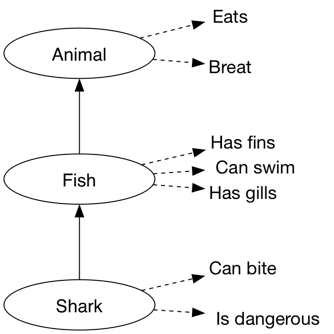
\includegraphics[width=0.60\textwidth]{MemoryStructure.png}
        \caption{A hypothetical memory structure, from \protect \citet{Collins1969}}
        \label{MemoryStructure}
    \end{center}
\end{figure}
 
% Chapter Template

\chapter{Methodology} % Main chapter title

\label{Methodology} % Change X to a consecutive number; for referencing this chapter elsewhere, use \ref{ChapterX}

\lhead{Chapter \ref{Methodology}. \emph{Methodology}} % Change X to a consecutive number; this is for the header on each page - perhaps a shortened title

The thesis utilizes the design research methodology to perform its research.
I will use the guidelines provided in \citet{Hevner2004} to ensure that the process is rigorous.
The guidelines provided in this article are:
\begin{enumerate}
	\item \label{gl1}Design as an Artifact
	\item \label{gl2}Problem Relevance
	\item \label{gl3}Design Evaluation
	\item \label{gl4}Research Contributions
	\item \label{gl5}Research Rigor
	\item \label{gl6}Design as a Search Process
	\item \label{gl7}Communication of Research
\end{enumerate}

I will now explain how I intend to follow these guidelines for the work related to this thesis.
The first guideline says that a design research project should produce some artefact.
Designing an artefact is central to this thesis.
I will use the system \theartefact\ to test my research question,
and the success of the system will decide whether the research question can be answered positively.

In the introduction I described my motivation for the thesis, and why it is a relevant contribution to design science.
I described the need for computer readable metadata for information retrieval,
and the difficultly inherent in the creation of this data for new users.
The work performed in completing this thesis can help lower the barrier of entry for generating semantically enriched websites.
If successful I hope to that the results can be used to both increase the value of computer search in general,
and increase the visibility and discoverability of the webpages that use tools that build on the work done.

Design evaluation is also mentioned and this guideline stresses the need for rigorous evaluation of the artefact that has been developed.
To evaluate the success of the project I will look at the artefacts ability to map natural language to ontologies.
The goal is to generate metadata that is of the level of quality as existing metadata of a comparable type.
I will also examine if it can add the metadata to the webpage using RDFa, without changing the way the webpage is rendered by browsers.

The main research contribution of this project will be \theartefact\,
which will contribute to solve the problem of how to get users to create semantic content.
This prototype system can serve, either as a starting point for development,
or as an inspiration as to how one can create a system that makes it easier to create semantic content on the web.

The need for research rigor, which is mentioned in guideline \ref{gl5} will be followed by following the multimethodological approach suggested in \citet{Chen1990} and \citet{NunamakerJr1990}.
\fig{MultiMethodological}{{A multimethodological approach to IS research, from \protect \citet{Chen1990}}}
\citet{Chen1990} proposes four activities for the design process that interact in the development of information systems
(see figure \ref{MultiMethodological} on page \pageref{MultiMethodological}).
The paper suggests using a multimethodological approach where one moves between different research activities:
Theory building, experimentation, observation and systems development.
By using these different approaches I hope that I will be able catch important facets that might otherwise have been missed or over looked.

Guideline \ref{gl6} says that design research should be a search process.
In this context that means that one should explore the possible implementations of the artefact by iterating through phases of
generating prototypes and testing these prototypes against the requirements of the project (as seen in figure \ref{GenerateTestCycle},
page \pageref{GenerateTestCycle}).
To attain this type of cycle I choose to use a system development methodology that utilizes multiple iterations of building and testing.

The last guideline proposed has to do with clear communication of the results of the research.
It is further proposed that one should take care to have several channels of communication with different levels of technical detail.
The reasoning is that one needs to convince both the technical and the managerial communities.

To conform to the seventh guideline one should communicate the results of ones research in such a way that it is accessible for the intended target audience.
The primary way of communicating the research will be this thesis.
The thesis will target an academic audience and describe the process of development,
and the evaluation of the artefact.

In addition the work done on the project is made available to the developer community,
with hopes that others can build on the work done in relation to this thesis.
All the source code from the project is open source,
developed and shared on GitHub\footnote{The project can be found at: \url{https://github.com/EivindEE/Madame}},
and released under the MIT license.
Releasing the source code of the project means that others can learn from the system in another way than what they
could just by reading this theses, as most of the details of implementation are outside the scope of an academic thesis.
It also means that all those who wish to improve upon the work,
either by resolving issues with the codebase or by adding new features,
can do so in a way that can enrich the tool for all those who wish to use it.

\fig{GenerateTestCycle}{{The generate/test cycle, from \protect \citet{Hevner2004}}}



% Chapter Template

\chapter{Findings} % Main chapter title

\label{Findings} % Change X to a consecutive number; for referencing this chapter elsewhere, use \ref{ChapterX}

\lhead{Chapter 4. \emph{Findings}} % Change X to a consecutive number; this is for the header on each page - perhaps a shortened title
 
% Chapter Template

\chapter{Analysis and Discussion} % Main chapter title

\label{AnalysisAndDiscussion}

\lhead{Chapter \ref{AnalysisAndDiscussion}. \emph{Analysis and Discussion}}

%----------------------------------------------------------------------------------------
%	Design Research
%----------------------------------------------------------------------------------------
\section{Comparing the algorithms}
\label{ComparingAlgorithms}
To compare the two algorithms we generated a list of english nouns
which we sent through the lexitags server to get synsets that corresponded to the meanings of each word.
Both these lists were preprocessed to remove duplicates and to format them as javascript objects
\footnote{\url{https://github.com/EivindEE/Madame/tree/master/testing}}.
The final list of synsets contained 4350 unique synsets.
We wrote a short script that we used to run the synsets through the best fit algorithms,
and write a report of the results.
For the schema.org version of the test we wrote the average depth of the mapped type,
as well as the total number of times the two algorithms had the same and different mappings.
The debth was calculated as the distance from the root node in the tree,
i.e. schema:Thing it self had a depth of 0,
schema:Person which inherits directly from schema:Thing has a depth of 1 and so on.
For the SUMO version the depth of each type was unavailable,
so we only have numbers showing the agreement between the algorithms.
The full results from the tests can be found at the URL \url{https://github.com/EivindEE/Master-thesis/tree/master/AlgComparison}.

As one can read from the numbers it table \ref{table:AlgorithmResults} the results from the SUMO test
display no difference between the two algorithms when mapping from WordNet to SUMO.
The two algorithms return identical mappings in 100\% of the test cases.
This indicates that there must have beena mapping either directly from the synset,
or from the direct hypernym of the synset for each of the 4350 synsets in our test.
This makes it hard to say anything relevant about the algoritms from these results.

The schema.org results are more interesting.
The two algorithms still perform fairly equally.
Reading from table \ref{table:AlgorithmResults} we can see that the algorithms are equal in 75\% of the cases,
but we can examine the 25\% that are different and see which perform better in those cases.
We can also see that the algorithms were unable to find a mapping in 13.7\% of the cases.
These cases can't tell us much about which algorithm we should prefere,
but could be a good starting point for finding parts of the WordNet to schema.org mapping which could be enhanced.

Our predictions beforhand was that the hypernymes first approach would have fewer incorrect mappings,
but would give results at a more shallow depth.
The last prediction was the easiest to test, as we know the schema.org hierarchy and can calculate the depth of each type.
For each mapping we registered the depth of the type in the schema.org hierarchy.
These depths were averaged over the total number of mappings made.

As seen in table \ref{table:AlgorithmComparison} both algorithms map fairly high in the hierachy.
The hypernymes first approach maps to a type at level 0.69 on average when considering all the synsets,
or to a type at level 0.72 when ignoring the cases where the two algorithms gave the same result.
As predicted the hypernym then siblings approach does a little better, though not much,
mapping to types at level 0.8, or 1.2 when excluding identical mappings.
Looking at the data it is obvious that the hyponymes first approach much more frequently leads to mappings to Thing and Intangible.
The hypernym first algorithm maps to schema:Thing 449, and schema:Intagible 481 times,
while hypernymes then siblings maps to schema:Thing 334 and schema:Intangible 81 times.
Neither schema:Thing nor schema:Intangible are very interesting mappings in the ontology.
As described in \ref{schemadotorg}, Thing is the most general category, meaning that every concept belongs to this category.
Intangible is described\footnote{\url{http://schema.org/Intangible}} as "a utility class that serves as the umbrella for a number of 'intangible' things",
and does not have any special properties in the ontology.
Even if these mappings are quite uninteresting it is not always obvious that there are types in schema.org which are better fits for the synsets.

To judge the correctness of the algorithms,
we went through the results from when the two algorithms gave different mappings and checked the mappings manually.
The process consisted of looking up each synset that was mapped,
and the types it had been mapped to and check if the two corresponded.
The results were divided into three categories.
If it was clear that the synset and type corresponded, they were marked as correct.
If it was clear that they didn't correspond they were marked as incorrect.
There were also some cases where it was unclear whether or not a mapping were correct.
These mappings included mapping bill\#n\#3("a piece of paper money"), to schema:Quantity("Quantities such as distance, time, mass, weight"),
where the description of schema:Quantity\footnote{\url{http://schema.org/Quantity}} further says
"Particular instances of say Mass are entities like '3 Kg' or '4 milligrams'",
making it unclear if a bill could be an instance of the schema:Quantity type even if it seems unnatural.

Since the manual inspection of the mappings was a time consuming process we decided to only inspect 250 mappings,
and see if the results of checking these would be sufficient to say anything about the algorithms.
We excluded mappings the schema:Thing and schema:Intangible, as one could normally argue reasonably for these.

We had predicted a higher error rate in the hypernym then sibling algorithm,
but the difference in the error rate between the algorithms was much larger than we had anticipated.
Again pointing to table \ref{table:AlgorithmComparison} we can see that the hypernyms first algorithm
made correct mappings in 96\% of the test cases,
while giving incorrect mappings in 0.8\% test cases and questionable mappings in 3.2\% of the cases.
The hypernym then sibling algorithm on the other hand gave a correct mapping in only 47.6\% of the cases checked.
It gave incorrect mappings in 45.6\% and unclear mappings in 7.2\% of the cases.
The fact that it gave correct mappings in less than 50\% of the instances where the results were different was very surprising.
This high degree of incorrect mappings indicates that using sibling synsets as the basis for mapping in unfruitful.
%%% EXPAND

The fact that the hypernyms first algorithm gave incorrect mappings at all are a bit alarming.
As described in section \ref{Hypernymy} about hyper- and hyponymy, hypernymy should be a transitive "type of" relation.
Each hypernym should then be a more general type of the synset provided and not break the semantics of the synset.
The mappings from WordNet to schema.org indicate that the semantic content of the synset are equal to the
semantic content of the schema.org type mapped to.
Since both hypernymy and mappings should preserve the semantics of the synsets, the mappings should be correct.
The fact that the hypernyms first algorithm gives incorrect mappings indicate that either the integrity of the hypernym relation is broken,
or that the mappings are incorrect.
The two cases where the hypernyms first approach gave incorrect mappings where with birth\#n\#1 and birthday\#n\#2,
which both mapped to schema:Quantity via their hypernym measure\#n\#2 \{measure, quantity, amount\}.

The hypernym chain linking birth\#n\#1 to measure\#n\#2 is:
\begin{verbatim}
	birth#n#1
	beginning#n#2
	point#n#6
	measure#n#2
\end{verbatim}

And from birthday\#n\#2:
\begin{verbatim}
	birthday#n#2
	date#n#1
	day#n#1
	time_unit#n#1
	measure#n#2
\end{verbatim}

The problem in both chains seem to be that one goes from something that happened at a single instance in time,
to a collection of things.
The there
%% Write more here

\begin{table}[h] %%%% Should I change the results so that the no results found are ignored?
	\centering
	\begin{tabular}{lll}
										& Schema.org	& SUMO			\\
		Total number of synsets tested 	& 4350			& 4350			\\
		Number of identical mappings 	& 3262 (75\%)	& 4350 (100\%)	\\
		Number  of different mappings	& 1088 (25\%)	& 0	(0\%)		\\
		No result found					& 598  (13.7\%)	& 0	(0\%)
	\end{tabular}
	\caption{The testing results}
	\label{table:AlgorithmResults}
\end{table}

\begin{table}[h]
	\centering
	\begin{tabular}{lll}
											& Hypernyms First 	& Hypernym then siblings	\\
		\emph{For all mappings}				&					&							\\
		Avg. depth total					& 0.688506 			& 0.804138					\\
		\emph{For different mappings}		&					&							\\
		Avg. depth different				& 0.721507			& 1.183823					\\
		Mappings to "Thing"					& 449				& 334						\\
		Mappings to "Intangible"			& 481				& 81						\\
		\emph{For the 250 examined mappings}&					&							\\
		Correct mappings					& 240				& 119						\\
		Correct mapping	rate				& 96\%				& 47.6\%					\\
		Unclear								& 8					& 18						\\
		Unclear	rate						& 3.2\%				& 7.2\%						\\
		Errors								& 2 				& 114 						\\
		Error rate							& 0.8\%				& 45.6\%					\\
	\end{tabular}
	\caption{Comparison of the mapping algorithms}
	\label{table:AlgorithmComparison}
\end{table}

Noun list from http://www.desiquintans.com/articles.php?page=nounlist

https://github.com/EivindEE/Master-thesis/blob/master/AlgComparison/AlgComparisonResultsBig
https://github.com/EivindEE/Master-thesis/blob/master/AlgComparison/compare-different
%----------------------------------------------------------------------------------------
%	Design Research
%----------------------------------------------------------------------------------------
\section{Suitability of WordNet for mapping natural language}
 
% Chapter Template

\chapter{Conclusion} % Main chapter title

\label{Conclusion} % Change X to a consecutive number; for referencing this chapter elsewhere, use \ref{ChapterX}

\lhead{Chapter 6. \emph{Conclusion}} % Change X to a consecutive number; this is for the header on each page - perhaps a shortened title
 

%----------------------------------------------------------------------------------------
%	THESIS CONTENT - APPENDICES
%----------------------------------------------------------------------------------------

\addtocontents{toc}{\vspace{2em}} % Add a gap in the Contents, for aesthetics

\appendix % Cue to tell LaTeX that the following 'chapters' are Appendices

% Include the appendices of the thesis as separate files from the Appendices folder
% Uncomment the lines as you write the Appendices

% Appendix A

\chapter{Appendix Title Here} % Main appendix title

\label{AppendixA} % For referencing this appendix elsewhere, use \ref{AppendixA}

\lhead{Appendix A. \emph{Appendix Title Here}} % This is for the header on each page - perhaps a shortened title

Write your Appendix content here.
%\input{./Appendices/AppendixB}
%\input{./Appendices/AppendixC}

\addtocontents{toc}{\vspace{2em}} % Add a gap in the Contents, for aesthetics

\backmatter

%----------------------------------------------------------------------------------------
%	BIBLIOGRAPHY
%----------------------------------------------------------------------------------------

\label{Bibliography}

\lhead{\emph{Bibliography}} % Change the page header to say "Bibliography"

\bibliographystyle{harvard} % Use the "unsrtnat" BibTeX style for formatting the Bibliography

\bibliography{Bibliography} % The references (bibliography) information are stored in the file named "Bibliography.bib"

\end{document}  
